\chapter{Konzept Client basierte Volume Manager Engine}
\label{cha:Konzept}

\section{Spezifikation}
\subsection{Objekte}
\subsubsection{Server}
Im folgenden wird der Volume Manager Verwaltungsserver als "'Server"' bezeichnet, welche den Client und deren Volume Manager verwaltet. Auf dem Server wird die eigentliche Logik und die Daten verwaltet. Die Daten der Disk und Volumes der einzelnen Clients werden auf dem Server in einer Datenbank gespeichert. Beim Anlegen eines neuen Volumes, werden die Informationen aus der Datenbank verwendet. 

\subsubsection{Client}
Als Client wird der zu verwaltende Server bezeichnet, auf welchem die Disks, die Volumes und das Filessystem verwaltet und konfiguriert werden sollen. Auf dem Client ist das Betriebsystem Linux mit dem Volume Manager LVM installiert. Für die Verwaltung des Client mittels Volume Manager Engine wird vorausgesetzt, dass der Client mit dem Server über TCP/IP kommunizieren kann. Mehrere Server zusammen können einen Cluster mit gemeinsamen Disk und Volumes bilden. Die einzelnen Servern können in verschiedenen Rechenzentren stehen.

\subsubsection{Speicher/Strorage}
Der Speicher kann eine im Server eingebaute Festplatte sein, oder der Speicher eines Storage-System, welches über eine Storage Area Network (\gls{SAN}) als LUN zugeordnet ist. Für eine Mirrored Volume ist es wichtig zu wissen, aus welchem Rechenzentrum das LUN stammt. Aus diesen Grund wird dem Speicher ein Ort bzw. ein Rechenzentrum zugeordnet

\subsubsection{Speichernetzt/Storage Area Network}
Über das Storage Area Network (\gls{SAN}) wir der Server mit dem Speichersystem verbunden.

\subsubsection{Ethernet Netzwerk}
Über das Ethernet Netzwerk kommuniziert der Server und die Clients miteinander.

\subsubsection{Standort/Site}
Als "'Site"' bezeichnen wir das Rechenzentrum. 

\subsubsection{Dateisystem/Filesystem}
Auf dem Logischen Volume wird ein Dateisystem erstellt, in welches die Daten gespeichert werden.

\subsubsection{Mountpoint}
Der Mountpoint ist der Pfad in welchem das Dateisystem eingehängt wird.

\subsubsection{Browser}
Der Webbrowser wird für den Dialog mit dem Anwender und für die Interaktion mit dem Volume Manager System verwendet.

\subsection{Annahmen}
Grundsätzlich ist es technisch möglich, Befehle für das Erstellen, Ändern und Löschen eines Clusters, einer Volume Group, eines Disk etc. direkt über das LVM oder via des neuen Tools vom Benutzer auszuführen. Für diese Arbeit wird angenommen, dass jedoch sämtliche Befehle durch das neue Tool erfasst werden, damit das Log-File lückenlos alle Befehle speichert und ausschliesslich mit den Daten aus der zentralen Datenbank für die anstehenden Mutationen gearbeitet wird. 
Würde diese Anforderung nicht erfüllt, so müsste angenommen werden, dass die Informationen zum System in der Datenbank nicht aktuell sind. Dann müsste vor jeder Mutationen das System, auf welchen die Mutation ausgeführt werden soll, neu eingelesen werden. Der Einlesevorgang kann bei Servern mit hoher Diskauslastung lange dauern und sich für den Benutzer als inakzeptabel auswirkt.


\subsection{Funktionen}

\subsubsection{Rollen und Benutzer}
Die Web-Applikation soll eine integrierte Benutzer- und Rollen-Verwaltung enthalten.
Um die Web-Applikation benützen zu können, muss man sich mit seinem persönlichen Benutzername und Passwort anmelden.

Beim Erfassen eines Benutzer muss dem Benutzer eine Rolle zugewiesen werden. Damit wird die Funktionsberechtigungen auf einfache Weise gesteuert.
Folgende Rollen werden von der Anwendung vorgeschlagen:

Admin
\begin{itemize}
\item Kann Benutzer erfassen und verwalten
\item Kann neue Server hinzufügen und abbauen
\item Kann neue Cluster hinzufügen und abbauen
\item Kann neue Volume Objekte auf einem Server/Cluster erstellen
\item Kann bestehende Volume Objekte auf einem Server/Cluster bearbeiten
\end{itemize}

System-Admin-Teamleader
\begin{itemize}
\item Kann neue Server hinzufügen und abbauen
\item Kann neue Cluster hinzufügen und abbauen
\item Kann neue Volume Objekte auf einem Server/Cluster erstellen
\item Kann bestehende Volume Objekte auf einem Server/Cluster bearbeiten
\item Kann nachvollziehen wer welche Mutationen durchgeführt hat
\end{itemize}

System-Admin
\begin{itemize}
\item Kann neue Server hinzufügen und abbauen
\item Kann neue Cluster hinzufügen und abbauen
\item Kann neue Volume Objekte auf einem Server/Cluster erstellen
\item Kann bestehende Volume Objekte auf einem Server/Cluster bearbeiten
\end{itemize}

System-Operator
\begin{itemize}
\item Kann neue Volume Objekte auf einem Server/Cluster erstellen
\item Kann bestehende Volume Objekte auf einen Server/Cluster bearbeiten
\end{itemize}

System-Operator-Teamleader
\begin{itemize}
\item Kann neue Volume Objekte auf einen Server/Cluster erstellen
\item Kann bestehende Volume Objekte auf einem Server/Cluster bearbeiten
\item Kann nachvollziehen wer welche Mutationen durchgeführt hat
\end{itemize}

Weitere Rollen aus der Anforderungsanalyse sollen zu einen späteren Zeitpunkt umgesetzt werden.

\subsubsection{Erfassen eines Clusters}
Neue Clusters sollen über ein Formular auf dem Webinterface erfasst werden können.
Beim Erfassen eines neuen Clusters, werden folgende Angaben benötigt.

\begin{itemize}
\item Clustername
\end{itemize}

\subsubsection{Erfassen eines Servers}
Neue Server sollen über eine Formular auf dem Webinterface erfasst werden können.
Beim Erfassen eines neuen Servers, benötigt es zwingend folgende Angaben:

\begin{itemize}
\item Servername
\item IP-Adresse\newline
\end{itemize}

Optional kann der Server einem Cluster als Mitglied zugeordnet werden. Sollte der Cluster noch nicht erfasst sein, soll es möglich sein an dieser Stelle diesen zu erfassen:

Nach dem Abspeichern der Serverinformationen, soll sich die Applikation mit dem Server verbinden, um das Betriebsystem, den installierten Volume Manager und alle vorhandenen LVM Objekte auszulesen.

\subsubsection{Einlesen der LVM Objekte}
 
Bei den Disks werden die folgenden Attribute eingelesen:
\begin{itemize}
\item Name
\item Grösse\newline
\end{itemize}

Bei den LUN werden folgende Attribute eingelesen:
\begin{itemize}
\item Name
\item Grösse
\item WWN\newline
\end{itemize}

Bei Physical Volume werden die folgenden Attribute eingelesen:
\begin{itemize}
\item Name
\item UUID
\item Grösse
\item Freier Speicher
\item Verwendeter Speicher
\item Anzahl Physical Volume Extents
\item Anzahl verwendeter Physical Volume Extents
\item Physical Volume Status
\item Volume Group UUID\newline
\end{itemize}

Bei Volume Group werden die folgenden Attribute eingelesen:
\begin{itemize}
\item Name
\item UUID
\item Grösse
\item Freier Speicher
\item Verwendeter Speicher 
\item Anzahl Volume Group Extents
\item Grösse der Volume Group Extents
\item Maximale Anzahl erlaubte Physical Volume
\item Maximale Anzahl erlaubte Logical Volume
\item Stauts der Volume Group\newline
\end{itemize}

Bei Logical Volume werden die folgenden Attribute eingelesen:
\begin{itemize}
\item Name
\item UUID
\item Grösse
\item Anzahl Extens
\item Berechtigung
\item Mirrorstatus
\item Volume Group UUID\newline
\end{itemize}

\subsubsection{Ausführen von LVM Mutationen}
Bei Mutationen an einem Clustermietglied soll die Konfiguration, wenn gewünscht, an allen Clustermitglieder vorgenommen werden

\subsubsection{Physical Volume erstellen}
Aus den zugeordneten leeren Volumes eines Servers bzw. Clusters sollen neue Physical Volumes über das Webinterface erstellt werden können.

\subsubsection{Volume Groups erstellen}
Aus einem oder mehreren freien Physical Volumes eines Servers bzw. Clusters soll über das Webinterface eine neue Volume Groupe erstellt werden können. Beim erstellen von Volume Groups soll zwischen Server Volume Group, einfachen Volume Group und hochverfügbaren Volume Group unterschieden werden können.

Bei Server Volume Groups können nur lokale Physical Volumes verwendet werden.

Bei einfachen Volume Groups können jeweils einzelne Physical Volumes unabhängig vom Standort verwendet werden. Der Benutzer soll beim Erstellen der Volume Groups erkennen können, aus welchem Standort die Physical Volumes stammen.

Bei hochverfügbaren Volume Groups können jeweils nur Physical Volumes in Paaren zugeordnet werden, wobei jeweils innerhalb eines Paares die Physical Volumes aus unterschiedlichen Standorten stammen müssen.

Einfache und hochverfügbare Volume Groups können clustered oder nicht clustered Volume Groups sein. 
Server Volume Groups können nur "'nicht Clustered Volume Groups"' sein.

\subsubsection{Volume Group erweitern}
Bestehenden Volume Groups sollen weitere Physical Volumes nach dem Schema zugeordnet werden können.

\subsubsection{Volume Group reduzieren}
Nicht mehr benötigter Speicherplatz soll bei Volume Groups mit dem Abbau von Physical Volumes wieder freigegeben werden können.

\subsubsection{Logical Volume erstellen}
Aus freien Extents einer Volume Group sollen über das Webinterface Logical Volumes erstellt werden können.

\subsubsection{Logical Volume Mirrored erstellen}
Aus freien Extents einer hochverfügbaren Volume Group sollen über das Webinterface Logical Volumes, welche gespiegelt sind, erstellt werden können.

\subsubsection{Logical Volume erweitern}
Bestehende Logical Volumes sollen durch Zuordnen von weiteren freien Extents aus der Volume Group erweitert werden können.

\subsubsection{Logical Volume reduzieren}
Bestehende Logical Volumes sollen durch entfernen von Extents verkleinert werden können.

\subsubsection{Report über alle freien Disks}
Mit einem Report über alle Servers bzw. Clusters sollen ungenutzte freie Disks angezeigt werden

\subsubsection{Report über alle freien Physical Volume}
Mit einem Report über alle Servers bzw. Clusters sollen ungenutzte freie Physical Volumes angezeigt werden

\subsubsection{Report durchschnittliche freie Extents pro Volume Group}
Mit einem Report über alle Servers bzw. Clusters soll der Durchschnitt aller freien Extents pro Volume Group angezeigt werden.

\subsubsection{Report über Mirrored Volumes}
Mit einem Report sollen alle ungespiegelte Logical Volumes ausgegeben werden.

\subsubsection{Report über alle nicht Multipath Luns}
Mit einem Report sollen alle Luns ausgegeben werden, welche nicht über zwei SAN-Verbindungen am Server angehängt sind.

\section{Architektur}
\begin{figure}
\centering
\includegraphics[width=1.1\textwidth]{Grundarchitektur.png}
\caption{Konzept: LVM Top-Level Architektur}
\label{fig:LVM Top-Level Architektur}
\end{figure}

\subsection{Programmiersprache}
Ruby ist eine interpretierte und objektorientierte Programmiersprache und beinhaltet einige bewährte Prinzipien wie z.B. "'DuckTyping"' und "'Principle of Least Suprice"'. Die Entwickler von Ruby stellen sich selber den Anspruch eine Programmiersprache zu schaffen, die durch Ihre Natürlichkeit einfach erlernbar ist und es den Programmierern ermöglicht, einfachen und übersichtlichen Code zu schreiben, welcher aber nicht seine Mächtigkeit und innere Komplexität verliert.
Ruby hat sich in den letzten Jahren von einer kaum beachteten Programmiersprache zu einem Publikums-Magneten entwickelt. Es gibt eine stetig wachsende offene Community "'Gemeinschaft"', welche sich und die Sprache durch Austausch von Erfahrungen und Ideen weiterbringen möchte.
Ein Grund für die hohe Bereitschaft der Community die Sprache Ruby weiter zu bringen ist der Umstand, dass die Programmiersprache vollständig OpenSource ist und unter der Lizenz der Ruby-License und GPL steht. Zudem ist die Sprache fast beliebig erweiterbar und bestehende Funktionen können einfach durch eigene Funktionen ausgetauscht werden.
Neben den oben genannten Vorteilen, gibt es sicherlich auch diverse Eigenschaften, welche im Vergleich zu anderen Sprachen gegen Ruby sprechen würden. Der hauptsächliche Grund die Sprache Ruby in diesem  Projekt einzusetzen, ist der Entscheid des aktuellen Arbeitgebers, bei möglichst allen neuen Projekten die Sprache Ruby einzusetzen.


\subsection{Web-Framework}
Das auf Ruby basierende Web-Framework Ruby on Rails auch "'Rails"' genannt, ist eines der beliebtesten Web-Framework für klein- bis mittelgrosse Anwendungen. Ruby on Rails wurde vom Dänen David Heinemeier Hannson geschrieben und gilt als Vorbild für weitere Web Applikations-Framework wie zB. Grails (Java), CakePHP (PHP), Django (Python) und "'softies on rails"' (.Net),  welche die Phylosophie von Rails übernommen haben. Wie die Programmiersprache Ruby ist auch das Framework OpenSource, steht jedoch unter der MIT License.

Alle Rails Applikationen unterliegen der gleichen Basisarchitektur. Die sich daraus ergebenden Vorteile liegen auf der Hand. Neue erfahrene Entwickler können sich rasch in ein neues Projekt einarbeiten, haben keine Mühe den bestehenden Code schnell zu erfassen und im Sinne der anderen Programmierer den Code weiterzuentwickeln. 

Rails Applikationen sind nach dem Design Pattern Model-View-Control (MVC) in drei Schichten unterteilt, die nachfolgend kurz besprochen werden sollen.

Model-Schicht
Die Model-Schicht entkoppelt die Daten von der Businesslogik zum Manipulieren von Daten.

View-Schicht
Die View-Schicht, auch Präsentationsschicht, stellt das User-Interface der Applikation dar. 

Controler-Schicht
Die Controller-Schicht ist verantwortlich, die Daten von der Benutzereingabe und externer Input zu interpretieren, indem sie mit dem beiden Schichten View und Model kommunizieren.

\begin{figure}[htb]
\centering
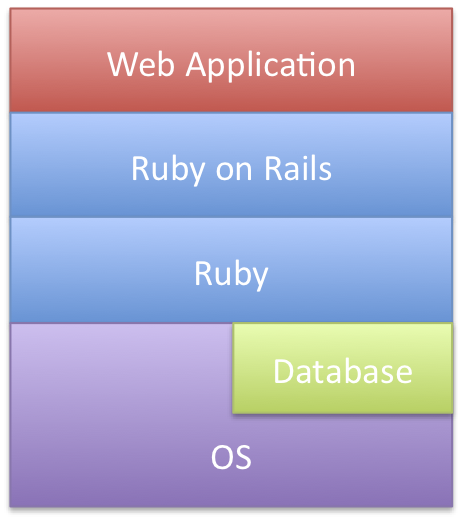
\includegraphics[width=0.5\textwidth]{RailsApplicationStack.png}
\caption{Rails Architektur: Applikation Stack}
\label{fig:Rails Applikation Stack}
\end{figure}
\nocite{Fisher200810}

Ruby On Rails ist nach den Architektur Stilen als Independent Components und Call-and-Return aufgebaut.

Als Independent Components besteht die Architektur aus unabhängigen Komponenten, welche wiederum aus unabhängig ablaufenden Elementen bestehen, die über Nachrichten miteinander interagieren. 

Bei Call-and-Return bzw. dessen Implementierung "'Layered"' werden sämtliche Elemente einzelnen Schichten zugeordnet, die hierarchisch geordnet sind. Jeder dieser Schichten erfüllt eine klar definierte Aufgabe.

Die Basis-Architektur wiederspiegelt sich auch in der Verzeichnisstruktur, welche bei allen Rails Applikationen gleich aufgebaut ist. 

\begin{itemize}
\item \textbf{app:} Hier befindet sich die eigentliche Rails Applikation in der MVC Struktur
\item \textbf{conf:} Applikation Konfigurationsdateien
\item \textbf{db:} Datenbank Schema und Migrations Dateien
\item \textbf{doc:} Dokumentation der Applikation
\item \textbf{lib:} Applicationsspezifischer Code, welcher nicht Teil des MVC Code ist
\item \textbf{log:} Applications Log
\item \textbf{public:} JavaScript, CSS, Bilder und andere statische Inhalte
\item \textbf{script:} Rails Scripts
\item \textbf{test:} Unit-test Code
\item \textbf{tmp:} Cache und Session Informationen
\item \textbf{vender: }Verwendete Fremd-Plugins
\end{itemize}


Neben der einheitlichen Dateistruktur und dem MVC Pattern, haben die Entwickler von Rails das Framework nach dem Design Pattern "'Don't Repeat Yourself"' (DRY) und "'Convention over configuration"' entwickelt.

\begin{figure}[htb]
\centering
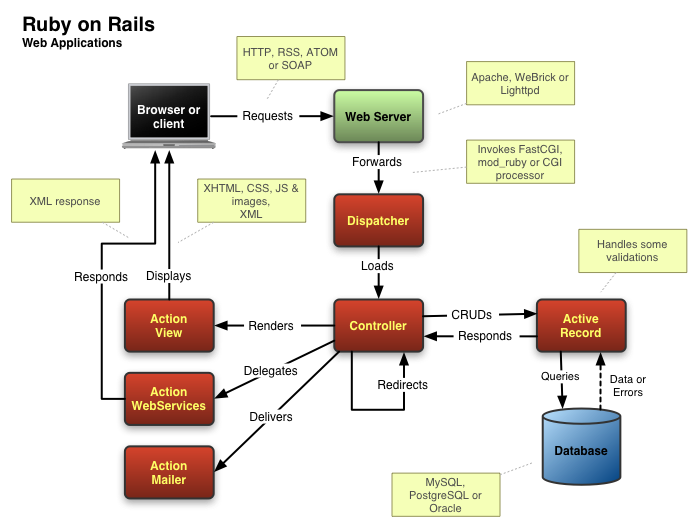
\includegraphics[width=1\textwidth]{rails_architecture.png}
\caption{Architektur: Ruby On Rails [http://blog.roi-office.com]}
\label{fig:RubyOnRails}
\end{figure} 

Die "'Don't Repeat Yourself"' Phylosophie geht davon aus, dass man sich bei der Entwicklung möglich nicht wiederholen soll und stattdessen einen generischen wiederverwendbaren Code entwickeln soll (projektoreintierte Entwicklung). 
Bei Rails wird die Phylosophie auf das ganze Framework angewendet, der Entwickler soll eine Definition nur an einem Ort vornehmen, ohne sich im Quelltext, in der Konfiguration oder in der Dokumentation wiederholen zu müssen. Durch diese vollständige Umsetzung von DRY erspart sich der Entwickler haufenweise Arbeit und verringert gleichzeitig die Fehleranfälligkeit seiner Applikation. Bei einer nachträglichen Anpassung z.B. eines Objekts, Funktion oder Konfiguration muss der Entwickler diese nur an einer Stelle anpassen. Ist der angepasste Quellcode genügend mit Unit-Test abgedeckt, muss der Entwickler bei dieser Anpassung nicht befürchten, dass er neue Fehler in die Applikation eingebaut haben könnte. Natürlich muss man bei diesem stark objektierten Konzeptansatz sich im klaren sein, dass in der Praxis in der Instanz viele Objekte entstehen können, die zwar ähnlich zu einem anderen Objekt sind, aber in dieser Ausprägung nicht weiter vererbt werden kann.

Eine weitverbreitete Eigenschaft von einem viel eingesetzten Applikations-Framework ist es, dass für die Verwendung des Frameworks grosse zum Teil komplexe Konfigurationen vorgenommen werden müssen. Mit der Philosophie "'Convention over configuration"' wollten die Rails Entwickler den Anwendern ihres Frameworks diese Arbeit ersparen. So verhält sich Rails in den meisten Fällen so, wie man es erwarten würde, ohne eine Spezifikation in einer Konfigurationsdatei vornehmen zu müssen.  So weiss z.B. der Routing Mechanismus von Rails ohne eine Konfiguration, welche Klasse und Methode den Seitenaufruf abhandeln muss. Wenn notwendig und gewünscht können diese Standardverhalten einfach überschrieben werden und geben dem Entwickler somit genügend Flexibilität.


\subsection{Datenmodell}

Das Datenmodell soll nach Möglichkeit die reale Welt abbilden, um die gegebenen Anforderungen und die Eigenschaften der Objekte im Datenmodell zu erfüllen. Es wurden folgende Überlegungen gemacht:

\begin{itemize}
\item Ein Cluster besteht aus mindestens zwei oder mehr Servern.
\item Ein Server kann Mitglied eines Clusters sein, oder stand-a-lone betrieben werden.
\item Für die Hochverfügbarkeit eines Clusters ist es wichtig zu wissen, in welcher Site ein Server steht. Aus diesen Grund ist ein Server immer einer Site zugeordnet.\newline
\end{itemize}


\begin{itemize}
\item Ein Server kann ein oder mehrere Volumemanger installiert haben.
\item Ein Server hat ein oder mehrere Disks, wobei es sich um Serverdisks oder LUN Disks handeln kann.
\item Ein Server kann Mitglied eines Clusters sein.
\item Ein Server hat ein oder mehrere Volumemanger
\item Ein Server befindet sich in einem Rechenzentrum/Site.
\item Ein Server hat ein oder mehre Disks.\newline
\end{itemize}


\begin{itemize}
\item Eine Disk kann ein Serverdisk oder LUN-Disk sein.
\item Eine Serverdisk ist immer einem Server zugeteilt. 
\item Eine LUN-Disk kann ein oder mehreren Servern zugeteilt sein.
\item Eine Disk wird nicht in Partitionen aufgeteilt.
\item Eine Disk kann für einen Volume-Manager verwendet werden.
\item Der Volumemanager bestimmt die dazugehörigen Objekte für die Disk.\newline
\end{itemize}


\begin{itemize}
\item Ein Physical Volume gehört immer einer Disk an.
\item Ein Physical Volume kann einer Volume Group zugeordnet werden.\newline
\end{itemize}


\begin{itemize}
\item Eine Volume Group besteht immer aus einer oder mehreren Physical Volumes.
\item Eine Voume Group kann eine oder mehrere Logical Volume Groups haben.\newline
\end{itemize}


\begin{itemize}
\item Ein Logical Volume gehört immer einem Volume Group an.
\item Ein Logical Volume hat eine Filesystem.\newline
\end{itemize}


\begin{itemize}
\item Ein Filesystem gehört immer einem Logical Volume an.
\item Ein Filesystem hat ein Mountpoint.\newline
\end{itemize}

Das im Abbild \ref{fig:Datenmodell} dargestellte Datenmodell, zeigt die Objekte und deren Verbindungen zueinander, zusätzlich enthält es eine mögliche Erweiterung für den Oracle ZFS Volume Manager.

\begin{figure}
\centering
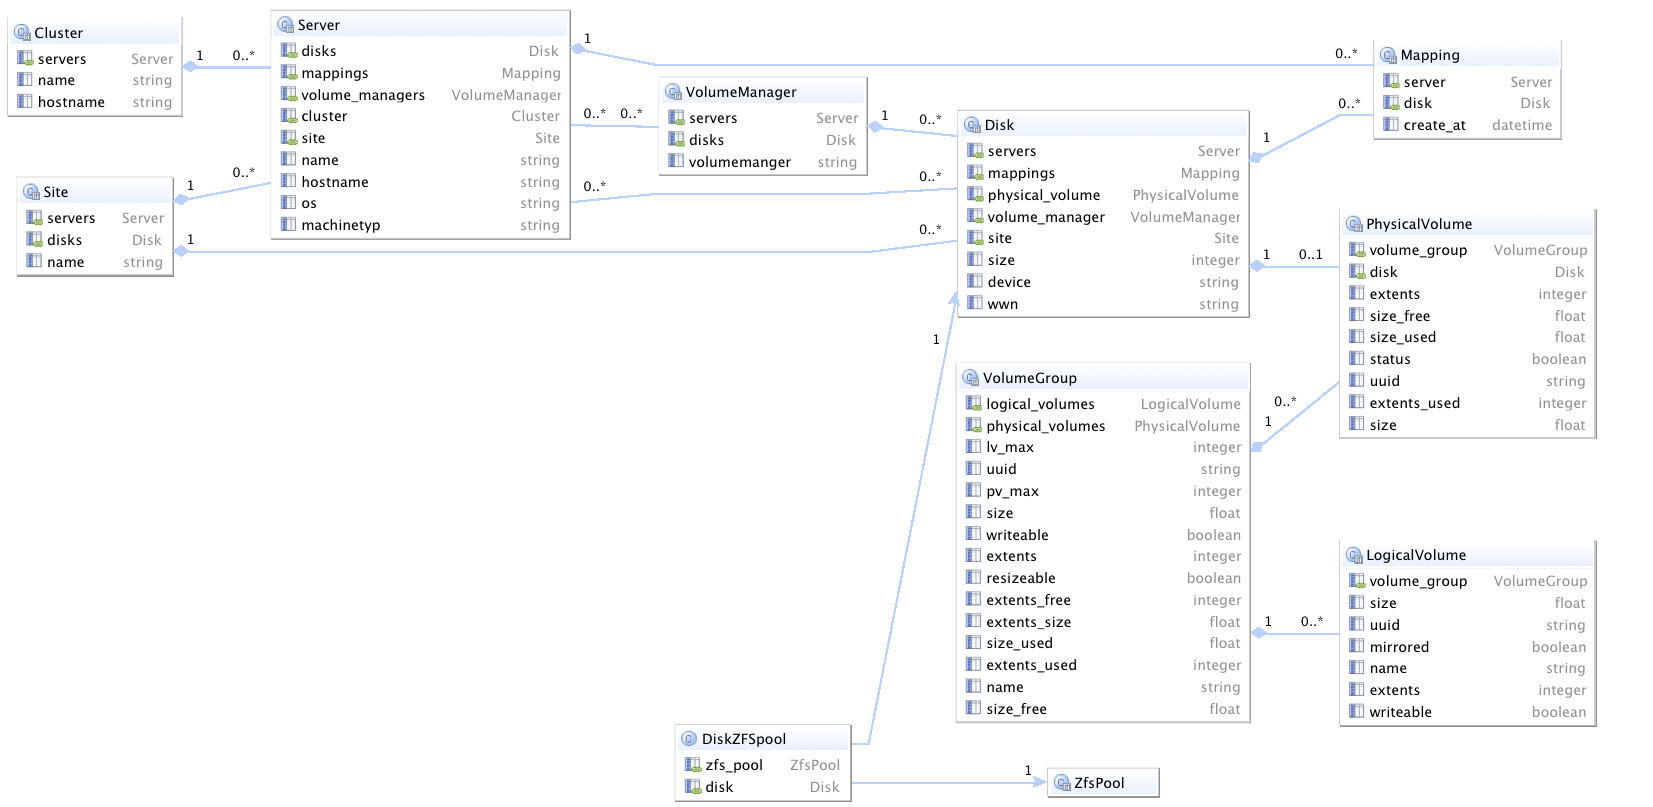
\includegraphics[width=1.5\textwidth, angle= 90]{DatenModell2.png}
\caption{Architektur: Datenmodell}
\label{fig:Datenmodell}
\end{figure}

\newpage
\subsection{LVM-Engine}
Die LVM-Engine inklusive Client-Server Kommunikation wird als Libary-Module für das Web-Framework umgesetzt. Somit ist die Logik der LVM-Engine vom Web-Framework gelöst und kann für andere Projekte wieder verwendet werden. 

\subsubsection{ruby-lvm-wrapper}

Das von den Entwicklern Matthew Kent und John Hampton  auf github veröffentlichte Projekt ruby-lvm-wrapper\footnote{\href{https://github.com/johnhampton/ruby-lvm}{https://github.com/johnhampton/ruby-lvm}} und dessen dazu gehörende Subprojekt ruby-lvm-attributes footnote\footnote{\href{http://rubyforge.org/projects/ruby-lvm-attrib/}{http://rubyforge.org/projects/ruby-lvm-attrib/}}, bietet eine gute Ausgangslage für die LVM-Engine.

Der LVM-\gls{Wrapper} des Projekts liest alle Logical Volumes, Logical Volume Segments , Volume Groups, Physical Volumes und Physical Segments aus einem lokalen Server aus und gibt diese als Ruby Objekt  zurück. Die Attribute der einzelnen LVM Objekten sind pro Objekt im \gls{YAML} Format definiert und in das separate Subprojekt ruby-lvm-attributes ausgelagert. Somit ist die Definition der Objekte vom eigentlichen Quellcode entkoppelt. Für jedes Attribut wird in der \gls{YAML} Datei eine \textit{\/:methode} mit dem LVM Attribute Namen, \textit{\/:type\_hint} mit dem Datentyp des Atttribues, \textit{\/:column} Name des Attributes im RubyObjekt und \textit{\/:description} mit der Beschreibung definiert. Ein Beispiel einer Definition wird in dem Listing \myref{lst:YAML} gezeigt. 
Von der LVM Version abhängig wird im ruby-lvm-attributes Projekt ein Gruppe von YAML Dateien für die Objekte erstellt.

\lstset{language=Ruby, basicstyle=\footnotesize, showstringspaces=false, tabsize=2}
\lstinputlisting[label=lst:YAML,caption=YAML: Beispiel Code aus \Code{PVS}]{DVD/Listings/pvsyaml.txt}

Für die Ausführung und das Auslesen der Ausgabe-Kanäle (englisch: streams), verwendet der Wrapper das \gls{API}  \gls{POpen4}\footnote{\href{https://github.com/pka/popen4}{https://github.com/pka/popen4}} von John-Mason und P. Shackelfords. POpen4 erstellt für die Ausführung der einzelnen Befehlen einen childprocess. POpen4 liest dabei die von POSIX Stream stdin, stdout und stderr aus.
\nocite{TomZrner}

\begin{itemize}
\item \textbf{stdin} ist der Eingabe-Kanal, meistens mit der Tastatur verbunden.
\item \textbf{stdout} ist der Ausgabe-Kanal einer Shell und wird normalerweise auf dem Terminal ausgegeben.
\item \textbf{stderr} ist der Fehler-Ausgabe-Kanal. Die Fehler werden standardmässig auf dem gleichen Gerät wie stdout ausgegeben.
\end{itemize}




\subsubsection{Anpassungen am ruby-lvm-wrapper}

Damit das Projekt ruby-lvm-wrapper die Anforderungen der LVM-Engine erfüllt, muss das Projekt angepasst und erweitert werden. Das Projekt wurde deshalb in einer Forke Version vom ursprünglichen Projekt abgespaltet.

Im ursprünglichen Ruby-lvm-wrapper Projekt, gibt es keinen Wrapper für die LVM Funktionen für das Erstellen und Modifizieren von LVM Objekten. Manipulationen sind zwar indirekt über die RAW Schnittstelle möglich, indem man die LVM Befehle der Schnittstelle übergibt. Dies bedeutet aber, dass die Logik ausserhalb der Ruby-lvm-wrapper zu implementieren ist. Die RAW-Schnittstelle wird deshalb im Forke durch weitere Wrappers für das Erstellen von Physical Volumes, Volume Groups und Logical Volumes ersetzt.

Das Auslesen von LVM Objekten und das Ausführen von Commandline Befehlen ist im ursprünglichen Ruby-lvm-wrapper Projekt auf den lokalen Rechner beschränkt. Die Ausführung im Fork wird mit einer Client-Server Software ersetzt bzw. ergänzt.

Ruby-lvm-wrapper prüft das System bei der Initialisierung auf die LVM Version des Systems und verwendet dazu je Version die YAML Dateien von Projekt ruby-lvm-attrib für das Auslesen der Objekt-Attribute. Weil pro Version die YAML Dateien vorhanden sein müssen,  birgt dies die folgenden Nachteile:
\begin{itemize}
\item Der Verwaltungsaufwand steigt mit der Anzahl der Versionen.
\item Die LVM-Engine könnte nach einer Aktualisierung eines Systems mit Patches, nicht mehr kompatibel (läuffähig) sein, wenn die Version von LVM wechselt.
\end{itemize}

Aus diesen Grund wird im Fork nur die im Datenmodell verwendeten Objekt-Attribute ausgelesen. Zusätzlich wird das Projekt ruby-lvm-attrib in den Fork integriert, was den Vorteil bringt, nicht mehr zwei Projekte parallel pflegen zu müssen.

Die Abbildung \myref{fig:Classdiagramm} zeigt das Klassendigramm nach der Anpassung.

\begin{figure}
\centering
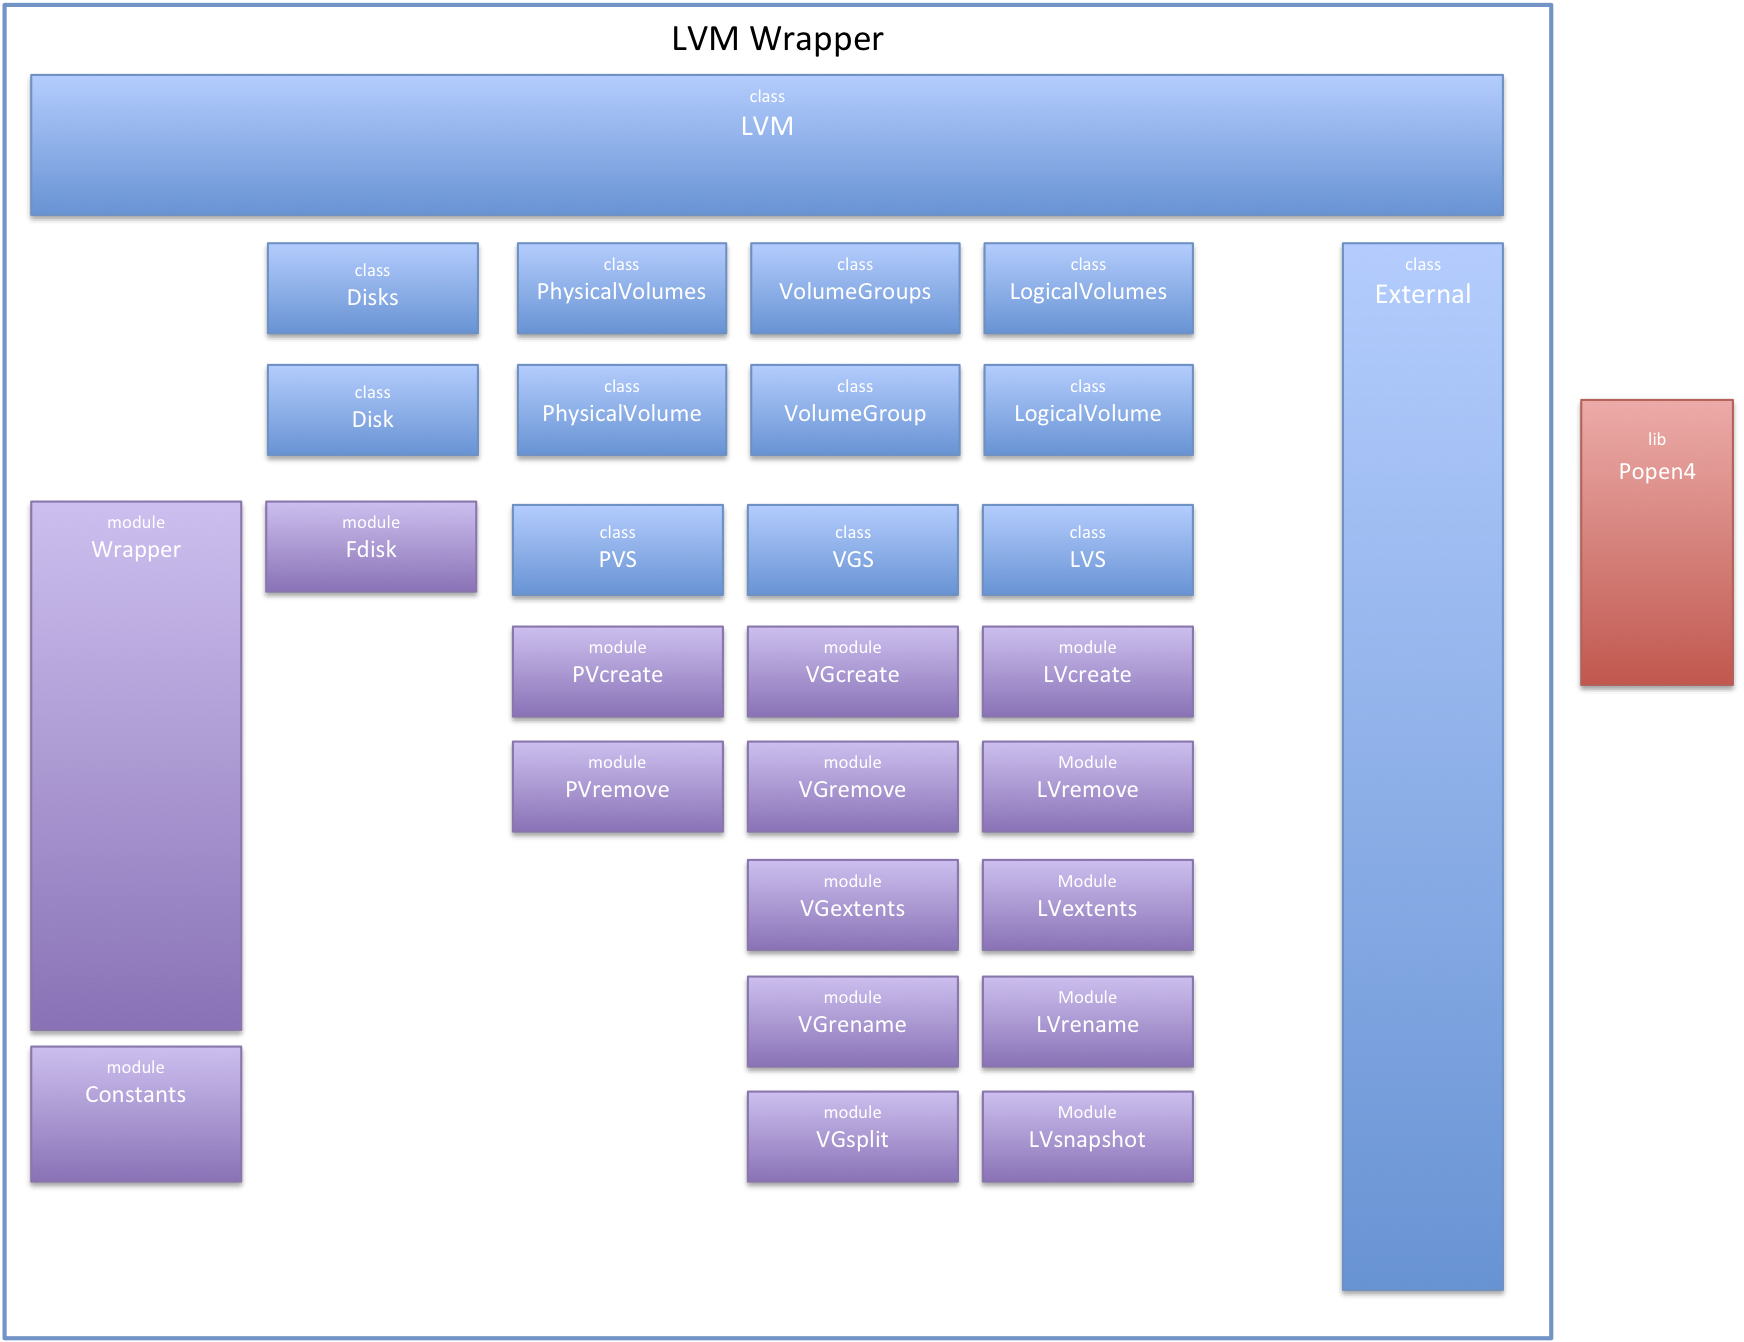
\includegraphics[width=1.5\textwidth , angle= 90]{ClassDiagramLVMWrapper.png}
\caption{Architektur: Klassendiagramm LVM Wrapper}
\label{fig:Classdiagramm}
\end{figure}

\subsection{Objekte Auslesen}
\subsubsection{Lokale Disk auslesen}
 
Die SCSI Disks, welche vom Linux-Kernel Ring erkennt werden, können mit \textit{dmesg} ausgelesen werden.

Befehl:\newline 
\Shell{ dmesg | grep "'SCSI device"' | uniq}
Ausgabe Beispiel:\newline
\Shell{SCSI device sda: 16777216 512-byte hdwr sectors (8590 MB)}

Aus der Ausgabe lässt sich der Gerätename (sda), die Sektorgrösse (512-byte), die Sektoren Anzahl (16777216) auslesen. Mit diesen Angaben lässt sich die Diskgrösse in byte berechnen.

\begin{equation}
Grösse In Byte = Sektorgrösse * Anzahl Sektoren
\end{equation}

\subsubsection{Physical Volumes auslesen}

LVM bietet die Möglichkeit, angepasste Reports der LVM Objekte auszugeben. Somit kann die Ausgabe optimal für das automatische Auslesen per Parser vorbereitet werden.

Befehl:\newline
\Shell{ pvs --separator="';"' --noheadings --nosuffix --units=b --unbuffered}
\Shell{ --options pv\_name,pv\_uuid,pv\_size,pv\_used,pv\_pe\_count,}
\Shell{ pv\_pe\_alloc\_count,pv\_attr,vg\_uuid}

Ausgabe Beispiel:\newline
\Shell{ /dev/sdb;hAL4Ok-vah7-V682-eQqh-n8Wj-geMA-JJKyqV;}
\Shell{ 213909504;0;51;0;a-;MTzZmV-yQua-cycm-msiv-fUM4-5718-wbUp1u}

Das Zeichen zwischen den einzelnen Attributen kann mit der Option --separator bestimmt werden. Bei der Ausgabe wird standardmässig eine Beschriftungzeile ausgegeben. Diese kann mit der Option --noheadings übersteuert werden. Die Einheit der Ausgabe kann mit der Option --units bestimmt werden. Für die Engine wird die Einheitsgrösse Bytes gewählt, somit werden keine kommaseparierten Zahlen ausgegeben.

\subsubsection{Volume Groups auslesen}

Befehl:\newline
\Shell{ vgs --separator=; --noheadings --nosuffix --units=b --unbuffered}
\Shell{ --options vg\_name,vg\_uuid,vg\_size,vg\_free,vg\_extent\_count,}
\Shell{ vg\_extent\_size,pv\_max,lv\_max,lv\_attr,vg\_uuid}

Ausgabe Beispiel:\newline
\Shell{ test;MTzZmV-yQua-cycm-msiv-fUM4-5718-wbUp1u;}
\Shell{ 213909504;213909504;51;4194304;0;0;wz--n-}

\subsubsection{Logical Volumes auslesen}


\Shell{ lvs --separator="';"' --noheadings --nosuffix --units=b --unbuffered}
\Shell{ --options lv\_name,lv\_uuid,lv\_size, pv\_used,pv\_pe\_count,}
\Shell{ pv\_pe\_alloc\_count,pv\_attr, vg\_uuid}



\subsection{Client-Server}
Die Client Server Komponente wird mittels Secure Shell (SSH) realisiert. Diese hat gegenüber einem proprietären Socket - oder einer XMLRPC Lösung den Vorteil, dass auf dem Client keine zusätzliche Software-Installation notwendig ist, die verteilt und später gewartet werden muss. Neue Anpassungen an der Software müssen nur auf einem zentralen Server installiert werden und vereinfacht somit den Versionenwechsel.

SSH gehört zu den Internet Standard Protokoll und ist unter den Request for Comments (\gls{RFC}) 4250\footnote{\href{http://www.ietf.org/rfc/rfc4250.txt}{http://www.ietf.org/rfc/rfc4250.txt}}, 4251\footnote{\href{http://www.ietf.org/rfc/rfc4251.txt}{http://www.ietf.org/rfc/rfc4251.txt}}, 4252\footnote{\href{http://www.ietf.org/rfc/rfc4252.txt}{http://www.ietf.org/rfc/rfc4252.txt}}, 4253\footnote{\href{http://www.ietf.org/rfc/rfc4253.txt}{http://www.ietf.org/rfc/rfc4253.txt}} und 4254\footnote{\href{http://www.ietf.org/rfc/rfc4254.txt}{http://www.ietf.org/rfc/rfc4254.txt}} standardisiert. Der SSH Server ist bei den wichtigen Linux Distributionen im Enterprice Umfeld standardmässig installiert und aktiviert. Mit SSH ist es möglich, auf einem entfernten Rechner bzw. Server, CLI befehle auszuführen, als würde man sich direkt am Terminal des Systems befinden.
Durch die relative einfach und sichere Nutzung, wird SSH von vielen Konfigurations-Applikationen verwendet, um Server zu verwalten.


\subsection{Kommunikation}
Das Anwendungs-Protokoll SSH kommuniziert über TCP auf dem Standard Port 22. Für die Kommunikation zwischen Server und Client sind keine weiteren Ports mehr nötig. Da SSH oft für die Server-Administration verwendet wird, ist dieser Port auf vielen Firewall geöffnet. Somit sind meist keine langwierigen Firewall Change-Requests notwendig.


\subsection{Sicherheit}
Mit dem Einsatz von SSH als Client-Server Komponente, ist durch die symmetrische Verschlüsselung mittels \gls{TrippleDES}, \gls{BlowFisch} oder \gls{AES} die Kommunikation sichergestellt. Damit sind keine Manipulationen beim Übertragen der Befehle auf den Client möglich. 

Für die Authentifizierung und den Schlüsselaustausch kann bzw. wird bei SSH das Public-Key Verfahren mittels \gls{RSA} eingesetzt. Mit diesem Verfahren ist sichergestellt, dass sich gleichzeitig nur ein Benutzer bzw. eine Applikation am System anmelden kann, wenn dieser im Besitz des privaten Schlüssels ist.


Für die Ausführung von LVM Befehlen auf dem System sind hohe Berechtigungsrechte auf dem System notwendig. Würde ein Angreifer Zugriff auf den Server erhalten, könnte er auf allen Clients Befehle mit hohen Rechten ausführen. Durch den Einsatz von \gls{SUDO} kann auf dem Client ein Benutzer mit niedrigen Rechten angelegt werden, welcher mit \gls{SUDO} nur die LVM-Befehle mit hohen Rechten ausführen kann.


\section{Testing}
Ein ausgereiftes white-box Testing hat einen spürbaren Einfluss auf die Code-Qualität. Ferner bietet es dem Entwickler die Möglichkeit, schneller auf Anforderungsänderungen einzugehen. Der Entwickler hat bei einem Projekt, bei welchem der Code gut mit Units-Test abgedeckt ist, bei Anpassungen am bestehenden Code eine gute Leitlinie, welche ihm hilft, weitgehend fehlerfrei zu entwickeln.
Für die Entwicklung des Projektes wird das in Ruby implementierte UnitTest Framework verwendet.

